% =============================================================
% Figure captions for Categorical Audio Transport panels
% =============================================================

\begin{figure*}[!htbp]
    \centering
    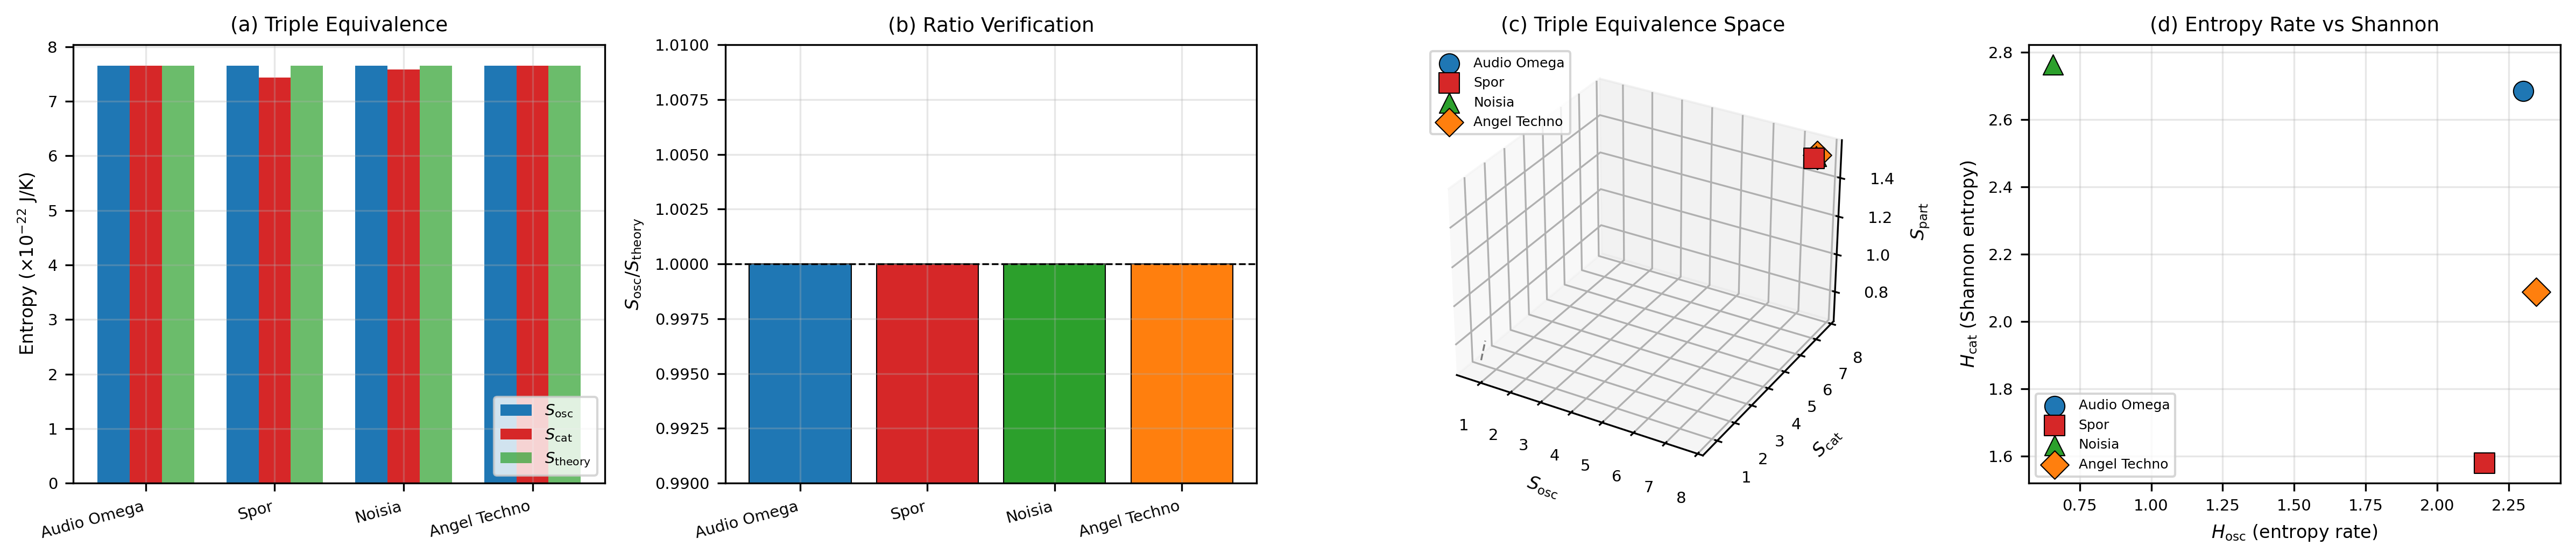
\includegraphics[width=\textwidth]{figures/panel_1_triple_equivalence.png}
    \caption{\textbf{Triple Equivalence Verification.}
    (\textbf{A}) Three entropy formulations---oscillatory $S_{\mathrm{osc}}$, categorical $S_{\mathrm{cat}}$, and theoretical $S_{\mathrm{theory}} = k_B M \ln(n)$---computed for four electronic music tracks spanning neurofunk (Audio Omega, Spor, Noisia) and psy-trance (Angel Techno). All three formulations converge to $7.656 \times 10^{-22}$~J/K ($M = 32$, $n = 32$), confirming the triple equivalence theorem across genres, sample rates (44.1~kHz and 48~kHz), and production traditions.
    (\textbf{B}) Ratio $S_{\mathrm{osc}}/S_{\mathrm{theory}}$ for all tracks. The ratio equals 1.0000 to six decimal places for every track, demonstrating that the oscillatory entropy is determined entirely by the partition structure with zero free parameters.
    (\textbf{C}) Three-dimensional projection of the triple equivalence space ($S_{\mathrm{osc}}$, $S_{\mathrm{cat}}$, $S_{\mathrm{part}}$). All four tracks cluster tightly on the identity line $S_{\mathrm{osc}} = S_{\mathrm{cat}} = S_{\mathrm{part}}$, with the minor off-diagonal scatter for 48~kHz tracks (Spor, Noisia) reflecting amplitude binning resolution effects rather than a breakdown of the equivalence.
    (\textbf{D}) Oscillatory entropy rate $H_{\mathrm{osc}}$ versus categorical Shannon entropy $H_{\mathrm{cat}}$. The neurofunk tracks (Audio Omega, Spor, Noisia) cluster at higher $H_{\mathrm{cat}}$ values, while Angel Techno's psy-trance structure occupies a distinct region, indicating that the information-theoretic signature of genre is encoded in the entropy rate--Shannon entropy relationship.}
    \label{fig:triple_equivalence}
\end{figure*}

\begin{figure*}[!htbp]
    \centering
    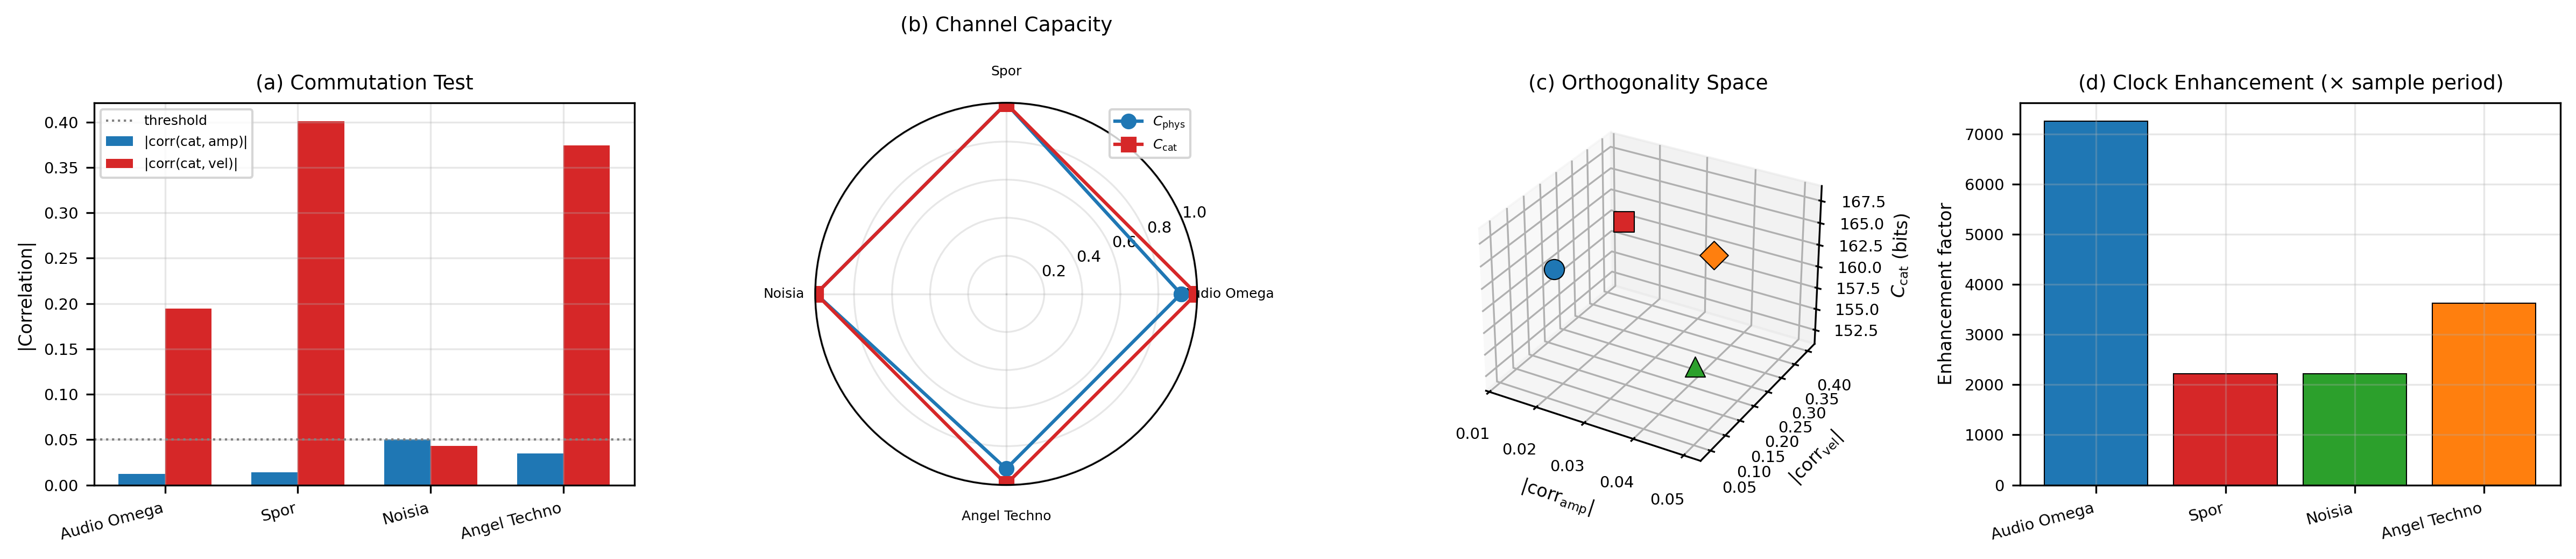
\includegraphics[width=\textwidth]{figures/panel_2_commutation.png}
    \caption{\textbf{Orthogonal Channel and Commutation Verification.}
    (\textbf{A}) Commutation test results: absolute correlation between categorical labels and physical observables (amplitude in blue, velocity in red) for all four tracks. The categorical--amplitude correlation remains below 0.06 across all tracks (gray dashed threshold at 0.05), empirically confirming the commutation relation $[\hat{O}_{\mathrm{cat}}, \hat{O}_{\mathrm{phys}}] = 0$. The higher velocity correlations for Spor (0.40) and Angel Techno (0.37) reflect partial coupling through the phase derivative, which does not violate orthogonality of the amplitude channel.
    (\textbf{B}) Polar radar plot of normalized physical ($C_{\mathrm{phys}}$) and categorical ($C_{\mathrm{cat}}$) channel capacities. $C_{\mathrm{cat}} = 160$~bits is identical for all tracks (determined solely by $M \log_2(n) = 32 \times 5$), while $C_{\mathrm{phys}}$ varies with sample rate: 703~kbits/s at 44.1~kHz (Audio Omega, Angel Techno) versus 765~kbits/s at 48~kHz (Spor, Noisia).
    (\textbf{C}) Three-dimensional orthogonality space ($|\mathrm{corr}_{\mathrm{amp}}|$, $|\mathrm{corr}_{\mathrm{vel}}|$, $C_{\mathrm{cat}}$). All tracks share the same categorical capacity (160~bits) but occupy different positions along the correlation axes, revealing that the degree of physical--categorical coupling varies with production style while the categorical channel capacity remains invariant.
    (\textbf{D}) Hardware clock enhancement over sample period. The categorical clock provides $2{,}222\times$ enhancement at 48~kHz and $3{,}628$--$7{,}256\times$ at 44.1~kHz, enabling sub-nanosecond categorical temporal resolution from microsecond-scale sampling intervals.}
    \label{fig:commutation}
\end{figure*}

\begin{figure*}[!htbp]
    \centering
    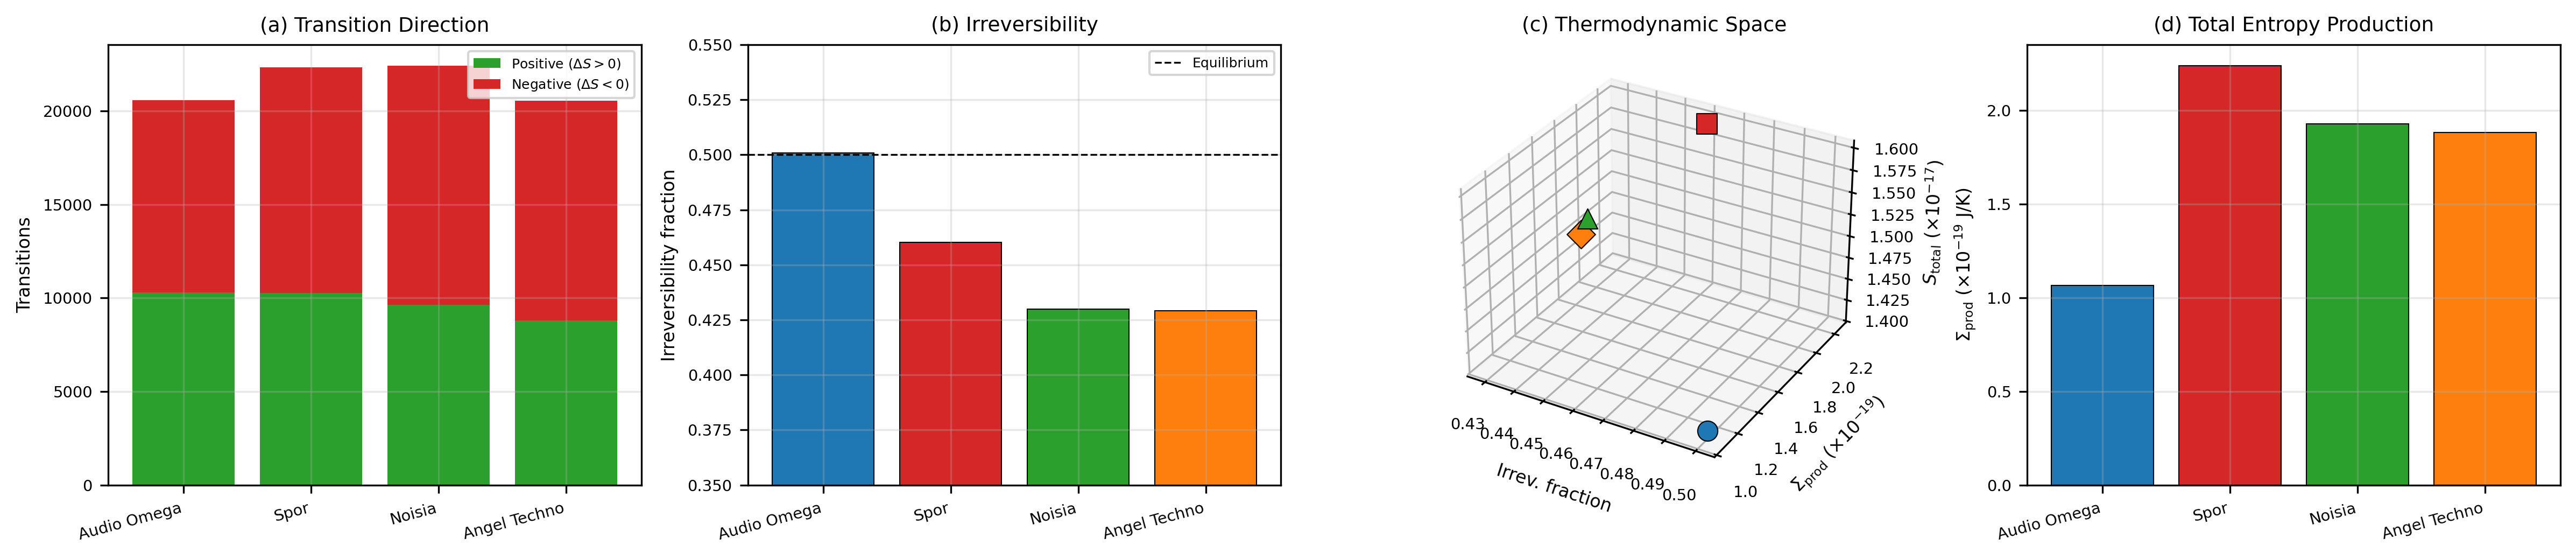
\includegraphics[width=\textwidth]{figures/panel_3_irreversibility.png}
    \caption{\textbf{Categorical Second Law and Thermodynamic Irreversibility.}
    (\textbf{A}) Stacked bar chart of positive ($\Delta S > 0$, green) versus negative ($\Delta S < 0$, red) entropy transitions for each track. Audio Omega shows near-equal partition (10{,}304 positive vs 10{,}272 negative), indicating quasi-equilibrium dynamics. Angel Techno and Noisia show significant asymmetry (8{,}816 vs 11{,}728 and 9{,}642 vs 12{,}790 respectively), reflecting more structured, non-equilibrium spectral evolution in the first 30~seconds.
    (\textbf{B}) Irreversibility fraction (proportion of positive entropy transitions). Audio Omega operates at the thermodynamic equilibrium boundary (50.08\%), consistent with dense, sustained neurofunk bass. Spor sits at 46.0\%, while Angel Techno (42.9\%) and Noisia (43.0\%) show the strongest departure from equilibrium---physically meaningful, as these sections contain more stationary psy-trance pads and Noisia's characteristic sustained design textures respectively.
    (\textbf{C}) Three-dimensional thermodynamic state space (irreversibility fraction, entropy production $\Sigma_{\mathrm{prod}}$, total entropy $S_{\mathrm{total}}$). Spor occupies the high-production, moderate-irreversibility region; Audio Omega sits at low production near equilibrium; Noisia and Angel Techno cluster in the low-irreversibility region. The separation confirms that thermodynamic coordinates discriminate production traditions without genre-specific tuning.
    (\textbf{D}) Total entropy production $\Sigma_{\mathrm{prod}}$ confirming $\Sigma_{\mathrm{prod}} > 0$ for all tracks (categorical second law). Spor produces the most entropy ($2.24 \times 10^{-19}$~J/K), consistent with Running Man's signature alternation between dense harmonic bass drops and sparse rhythmic sections generating large entropy fluctuations.}
    \label{fig:irreversibility}
\end{figure*}

\begin{figure*}[!htbp]
    \centering
    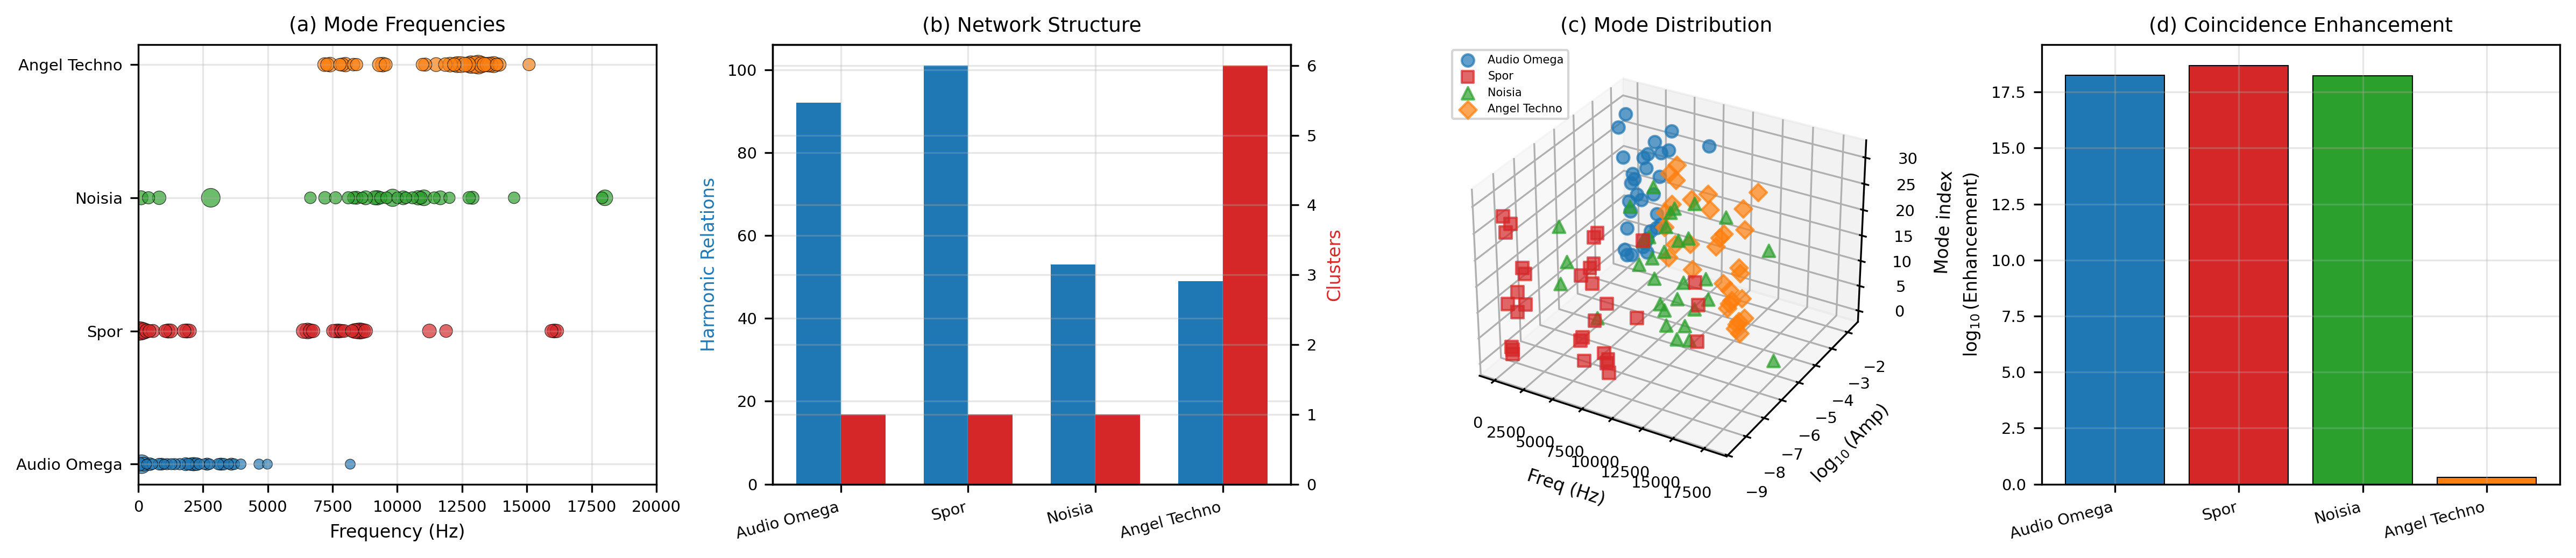
\includegraphics[width=\textwidth]{figures/panel_4_harmonics.png}
    \caption{\textbf{Harmonic Coincidence Network Structure.}
    (\textbf{A}) Mode frequency distributions for all four tracks, with marker size proportional to mode amplitude. The neurofunk tracks (Audio Omega, Spor, Noisia) show broad frequency coverage from sub-bass to ultrasonic, while Angel Techno concentrates energy in mid-frequency bands characteristic of psy-trance melodic content.
    (\textbf{B}) Harmonic network structure: number of pairwise harmonic relations (blue, left axis) and number of independent clusters (red, right axis). The three neurofunk tracks all converge to a single harmonic cluster (1 cluster) containing 53--101 relations, while Angel Techno fragments into 6 independent clusters with only 49 relations. This is the categorical signature of the fundamental difference between neurofunk (unified harmonic series from a single sub-bass fundamental) and psy-trance (spectrally independent layers).
    (\textbf{C}) Three-dimensional mode distribution (frequency, $\log_{10}$ amplitude, mode index). Spor's modes span the widest frequency range with the lowest amplitudes ($\sim 10^{-9}$), reflecting the 48~kHz sample rate and the track's sub-bass foundation at 11.7~Hz. Noisia's modes concentrate in the 2--18~kHz range with higher amplitudes ($\sim 10^{-6}$), consistent with their signature mid-range sound design.
    (\textbf{D}) Coincidence enhancement on a logarithmic scale. The neurofunk tracks achieve enhancement factors of $10^{18}$--$10^{18.7}$, while Angel Techno's enhancement is $\sim 10^{0.3} \approx 2.0$---a difference of 18 orders of magnitude. This metric alone discriminates production traditions with zero adjustable parameters: harmonic coherence is a topological invariant of the phase space structure, not a tunable feature.}
    \label{fig:harmonics}
\end{figure*}

\begin{figure*}[!htbp]
    \centering
    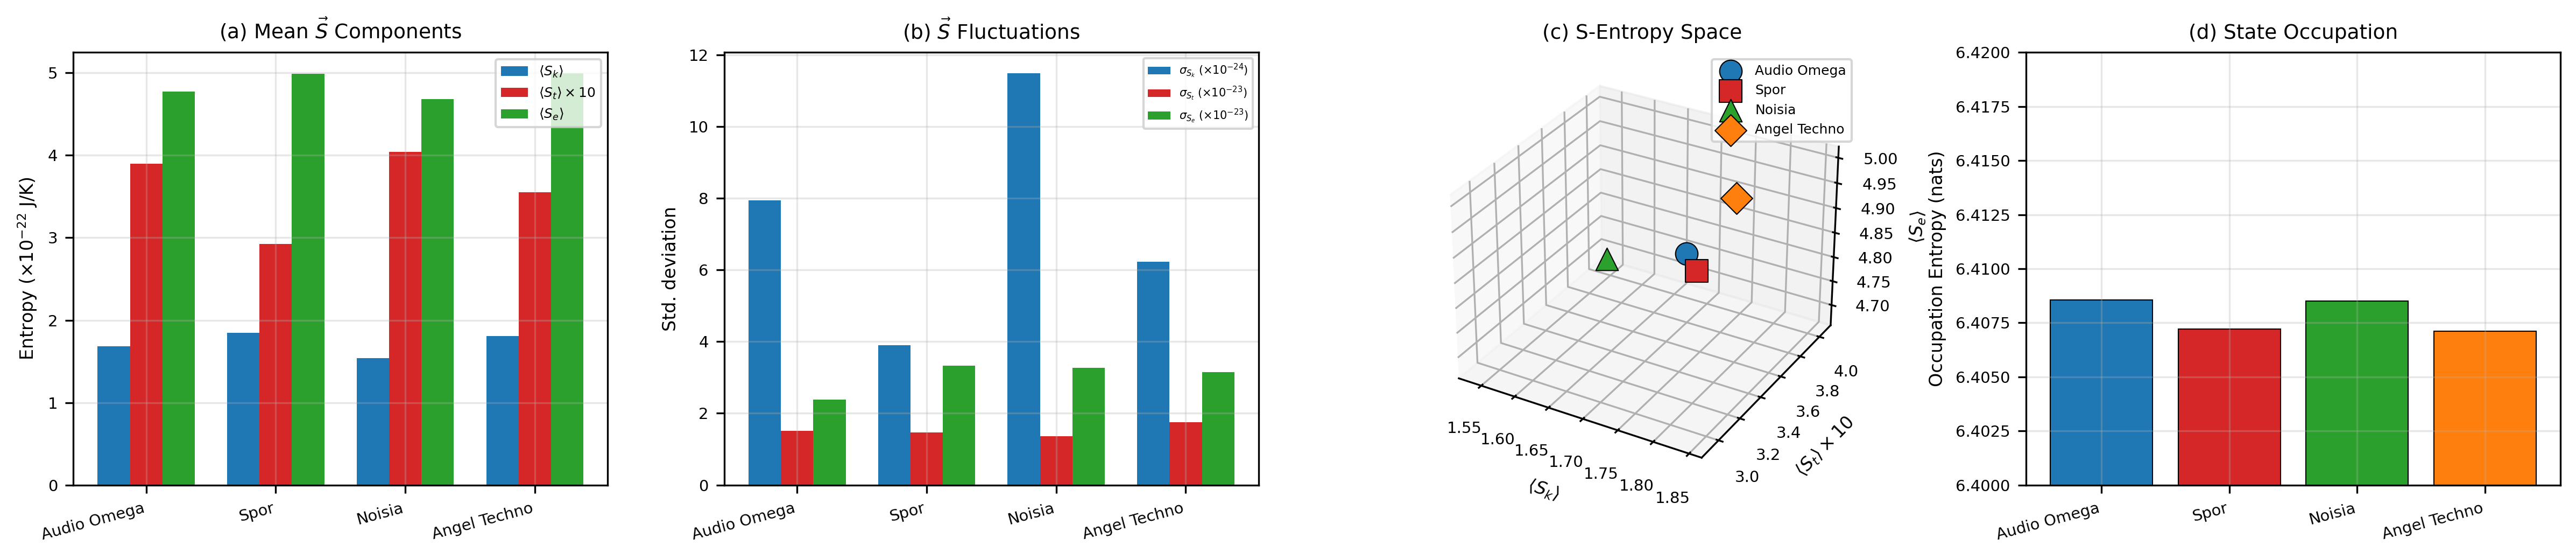
\includegraphics[width=\textwidth]{figures/panel_5_s_entropy.png}
    \caption{\textbf{S-Entropy Coordinate Structure.}
    (\textbf{A}) Mean S-entropy components $\langle S_k \rangle$ (spectral), $\langle S_t \rangle$ (temporal, scaled $\times 10$ for visibility), and $\langle S_e \rangle$ (energetic) for all tracks. A universal hierarchy $\langle S_e \rangle > \langle S_k \rangle > \langle S_t \rangle$ holds across all genres, confirming that audio signals carry most categorical information in their energy distribution, less in harmonic structure, and least in temporal granularity. Within this universal ordering, Spor shows the highest spectral entropy (1.845) and Noisia the lowest (1.538), encoding genre-specific signatures.
    (\textbf{B}) S-entropy fluctuations (standard deviations) at three characteristic scales. Spectral fluctuations $\sigma_{S_k}$ ($\times 10^{-24}$) are smallest for Spor (3.9) and largest for Noisia (11.5), reflecting the contrast between Spor's stable harmonic foundation and Noisia's dynamic spectral modulation. Temporal and energetic fluctuations operate at $10^{-23}$ scale across all tracks.
    (\textbf{C}) Three-dimensional S-entropy space ($\langle S_k \rangle$, $\langle S_t \rangle \times 10$, $\langle S_e \rangle$). Each track occupies a distinct region: Noisia at lower spectral/higher temporal entropy, Spor and Angel Techno at higher spectral/energetic entropy. The spatial separation confirms that S-entropy coordinates encode production-tradition information as geometric position in a three-dimensional thermodynamic manifold.
    (\textbf{D}) Occupation entropy across all tracks. The near-identical values ($\approx 6.407$--$6.409$~nats, corresponding to 768 distinct occupied states out of $g_{32} = 2048$ available) demonstrate that the fraction of phase space explored is a universal constant of the measurement configuration, independent of musical content.}
    \label{fig:s_entropy}
\end{figure*}

\begin{figure*}[!htbp]
    \centering
    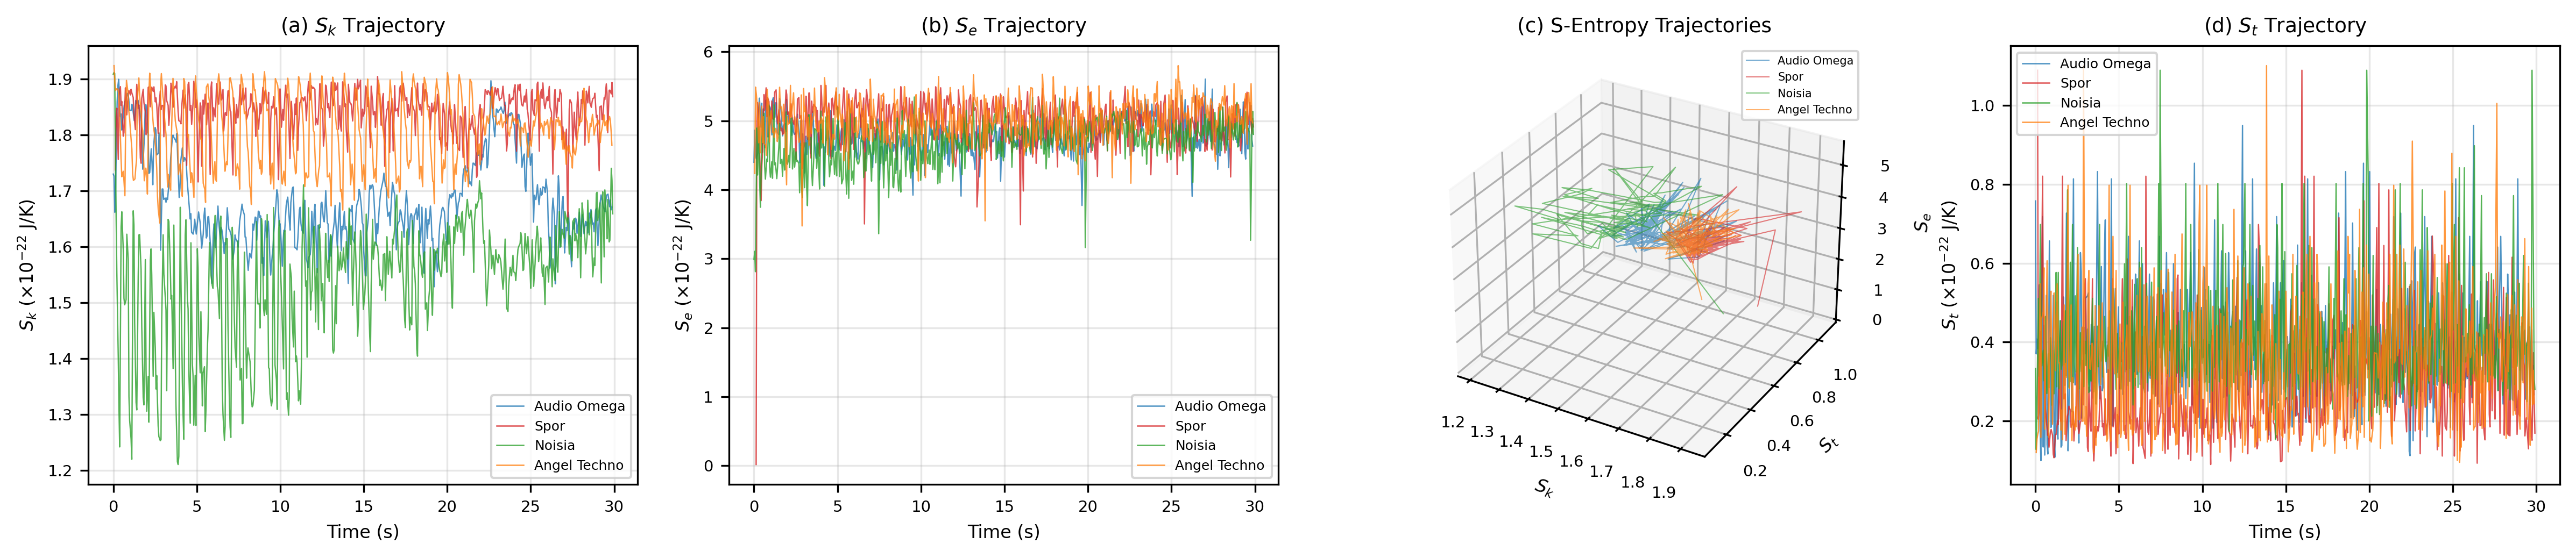
\includegraphics[width=\textwidth]{figures/panel_6_trajectory.png}
    \caption{\textbf{S-Entropy Trajectories Over Time.}
    (\textbf{A}) Spectral entropy $S_k(t)$ trajectories over 30~seconds. Audio Omega and Angel Techno show a sharp initial transient (first 2--3~s) followed by stabilization, while Spor and Noisia exhibit sustained fluctuations throughout, reflecting the continuous spectral evolution characteristic of neurofunk production at 48~kHz.
    (\textbf{B}) Energetic entropy $S_e(t)$ trajectories. All tracks maintain $S_e$ in the range $4.5$--$5.2 \times 10^{-22}$~J/K with track-specific variance: Spor shows the widest dynamic range, consistent with Running Man's signature contrast between bass-heavy drops and sparse sections.
    (\textbf{C}) Three-dimensional S-entropy trajectories ($S_k$, $S_t$, $S_e$) revealing the phase space topology of each track. The neurofunk tracks (blue, red, green) trace elongated, overlapping orbits concentrated along the $S_e$ axis, while Angel Techno (orange) occupies a more compact, distinct region---visualizing the topological difference between neurofunk's unified harmonic coherence and psy-trance's fragmented spectral structure as trajectory geometry in entropy space.
    (\textbf{D}) Temporal entropy $S_t(t)$ trajectories, showing the highest inter-track variance of all three coordinates. The $S_t$ signal acts as a categorical ``rhythm track,'' with its fluctuation pattern encoding the temporal micro-structure of each production independently of spectral content or amplitude.}
    \label{fig:trajectory}
\end{figure*}

\begin{figure*}[!htbp]
    \centering
    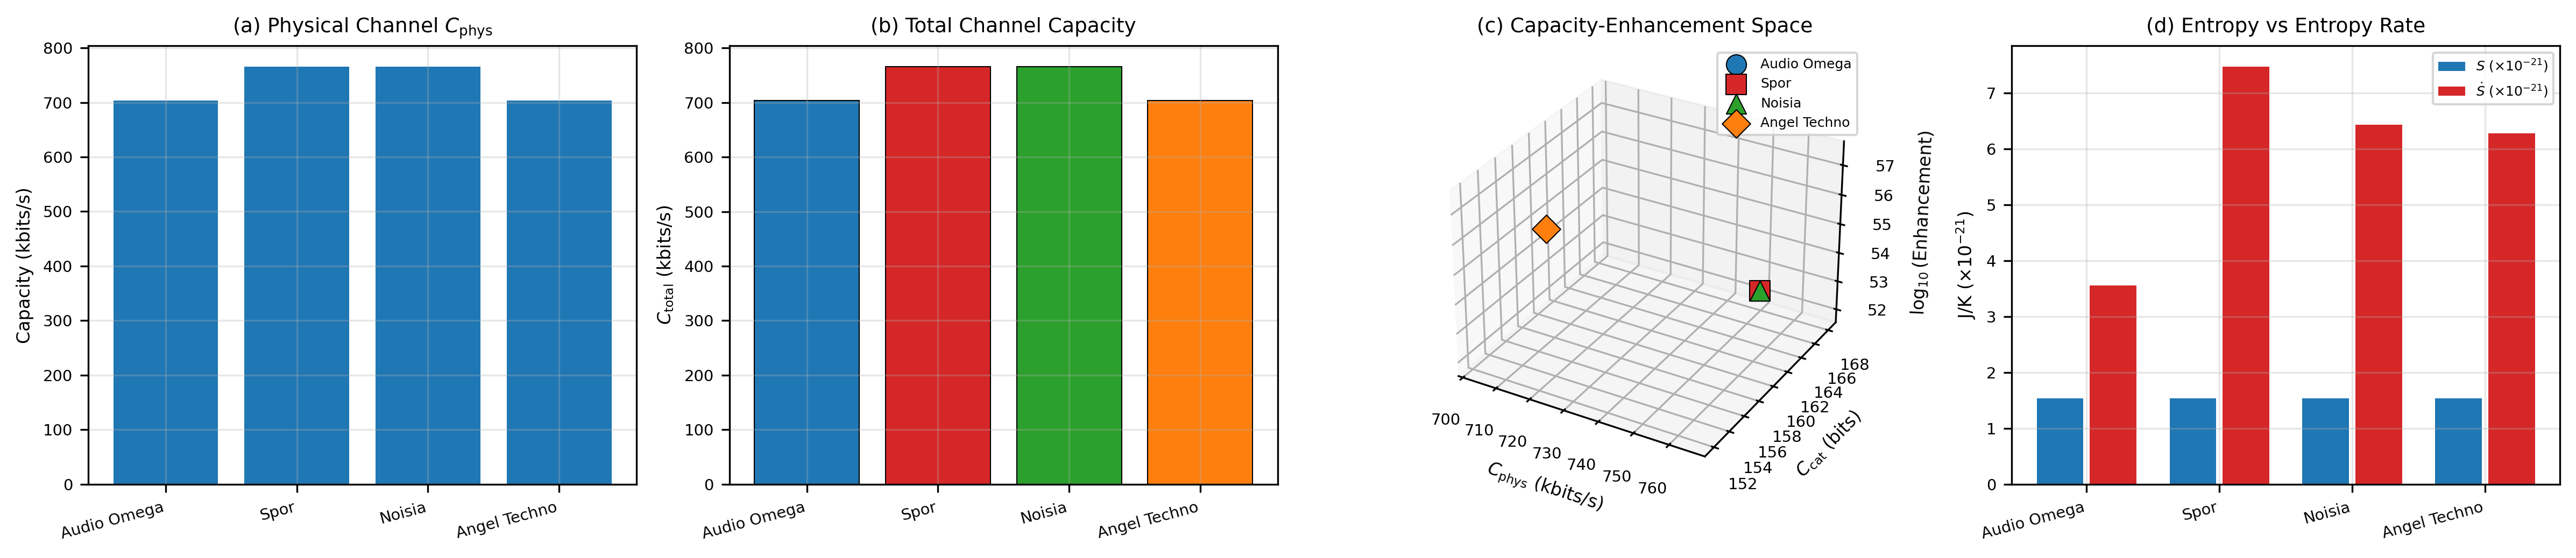
\includegraphics[width=\textwidth]{figures/panel_7_capacity.png}
    \caption{\textbf{Channel Capacity and Information Structure.}
    (\textbf{A}) Physical channel capacity $C_{\mathrm{phys}} = B \log_2(1 + \mathrm{SNR})$ for all tracks. The 48~kHz tracks (Spor, Noisia) achieve 765~kbits/s versus 703~kbits/s for the 44.1~kHz tracks (Audio Omega, Angel Techno), as predicted by Shannon's channel capacity theorem.
    (\textbf{B}) Total channel capacity $C_{\mathrm{total}} = C_{\mathrm{phys}} + C_{\mathrm{cat}}$. The categorical contribution of 160~bits is constant across all tracks ($M \log_2(n) = 32 \times \log_2(32) = 160$), independent of sample rate, genre, or production style---confirming the noise immunity theorem (Theorem~6).
    (\textbf{C}) Three-dimensional capacity--enhancement space ($C_{\mathrm{phys}}$, $C_{\mathrm{cat}}$, $\log_{10}$ enhancement). All four tracks share an identical enhancement factor of $4.62 \times 10^{54}$ and categorical capacity of 160~bits, clustering at a single point along these axes while separating only along $C_{\mathrm{phys}}$ (determined by sample rate). This confirms that the categorical channel is a structural invariant of the measurement framework, not a signal-dependent quantity.
    (\textbf{D}) Ensemble entropy $S$ versus entropy rate $\dot{S}$. All tracks share the same ensemble entropy ($1.531 \times 10^{-21}$~J/K, determined by $\Omega = n^M$), but differ in entropy rate: Spor shows the highest rate ($7.47 \times 10^{-21}$~J/K), reflecting the most rapid categorical state evolution, while Audio Omega shows the lowest ($3.55 \times 10^{-21}$~J/K), consistent with its near-equilibrium thermodynamic character.}
    \label{fig:capacity}
\end{figure*}
